% @Author: AnthonyKenny98
% @Date:   2020-02-23 14:27:21
% @Last Modified by:   AnthonyKenny98
% @Last Modified time: 2020-04-11 00:47:46

\subsection{Project Goals}
This is not the first project to attempt to accelerate motion planning algorithms using hardware; motion planning optimization has been studied extensively in hardware and in software. But the problem persists that, due to the nature of conventional \glspl{ISA}, there are significant barriers to implementing motion planning specific processors. \\

RISC-V was released 9 years ago. While it is starting to gain some traction in the commercial space, RISC-V has not yet been used to develop a motion planning specific processor. As such, the overall mission of this thesis is as follows:

\begin{center}
\bigskip\noindent\fbox{
    \parbox{0.8\textwidth}{
    \begin{center}
        \textbf{Mission} \\
        To present a proof-of-concept for extending and implementing RISC-V to develop motion planning specific processors.
    \end{center}
    }
} \\
\end{center}

\noindent To achieve this, the following 4 objectives must be accomplished:

\begin{center}
\bigskip\noindent\fbox{
    \parbox{0.9\textwidth}{
        \begin{center}        
        \textbf{Project Objectives} \\
        \end{center}
        \begin{enumerate}
            \item Determine the computational bottleneck of a commonly used motion planning algorithm.
            \item Implement a functional hardware module to replace the bottleneck function.
            \item Define a motion planning extension to the RISC-V ISA 
            \item Build a fully functional motion-planning processor that implements the extended RISC-V ISA
        \end{enumerate}
    }
} \\
\end{center}

    \newpage
    \subsubsection{Computer Implementation Hierarchy}
        To briefly frame the space in which this thesis operates, consider the hierarchy of computer implementation, demonstrated in Figure \ref{fig:computerHierarchy}. \textbf{User level applications}, such as Microsoft Word, Google Chrome, and Apple's iTunes, sit at the top of the hierarchy. These applications are implemented in \textbf{High/Mid Level Languages}, such as C/, C++, Python, Java, etc. 
        This software is eventually executed on a \textbf{Processor}, otherwise known as a \gls{CPU}. A processor does not understand Python, or any other programming language for that matter. The only thing it can understand is binary values (a one or a zero). Every computer program gets translated into ones and zeros (called machine code) for execution on a processor. But how are languages like C translated into machine code? The layer between programming languages and the processor is the \textbf{Instruction Set Architecture (ISA)}. Chapter 4 goes into detail about \gls{ISA}s and how they work. For now, if unfamiliar with the topic, it is sufficient to think of an \gls{ISA} as a translator between programming languages and machine code. This thesis operates across the lower three levels of this hierarchy.
        
        % @Author: AnthonyKenny98
% @Date:   2020-02-29 23:52:30
% @Last Modified by:   AnthonyKenny98
% @Last Modified time: 2020-04-10 12:37:43
\begin{figure}[H]
\begin{center}
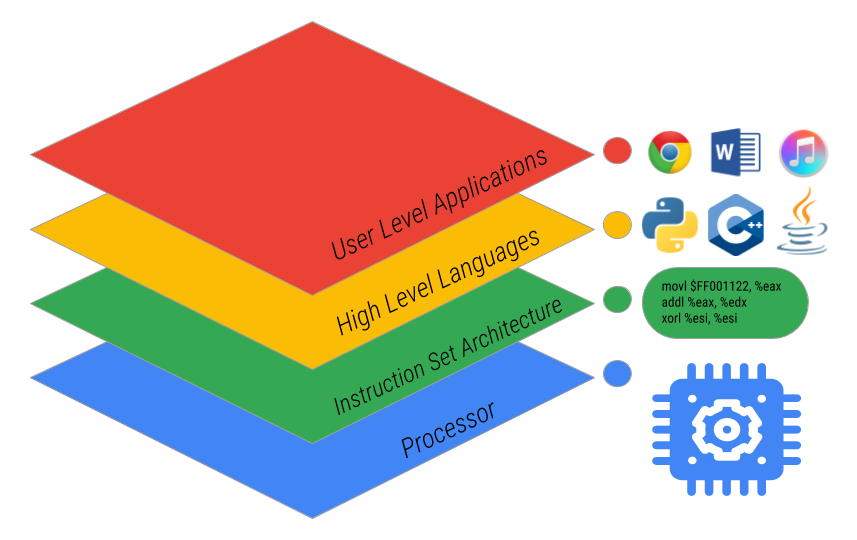
\includegraphics[width=\linewidth]{chapters/chapter1/img/computerHierarchy.png}
\mycaption{Simple Visualization of Computer Implementation Hierarchy}{}
\label{fig:computerHierarchy}
\end{center}
\end{figure}



\subsection{Project Structure}
\label{subsection:project_structure}

    Chapter 2 details how \glsfirst{RRT}, a commonly used motion planning algorithm, is implemented and analysed. From this analysis, it was determined that the computational bottleneck is edge collision detection. Chapter 3 outlines a process for implementing this bottleneck function in a hardware module, achieving a $5 \times$ speedup. Chapter 4 defines the RISC-V motion planning extension and describes the build of a RISC-V processor that implements this extension and the Honeybee unit.


    \subsubsection{System Overview}
        Figure \ref{fig:systemDiagram} shows a high level overview of the system this thesis proposes.
        % @Author: AnthonyKenny98
% @Date:   2020-03-01 11:14:04
% @Last Modified by:   AnthonyKenny98
% @Last Modified time: 2020-03-01 11:45:10
\begin{figure}[H]
\begin{center}
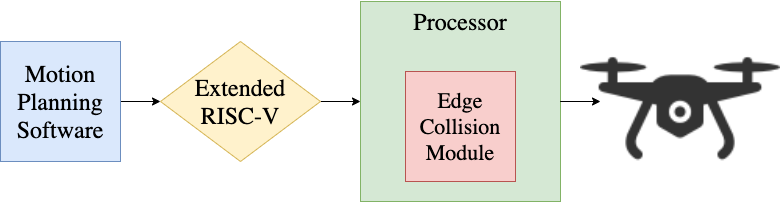
\includegraphics[width=\linewidth]{chapters/chapter1/img/systemDiagram.png}
\caption{System Diagram of Overall Project}
\label{fig:systemDiagram}
\end{center}
\end{figure}

        Table \ref{table:componentList} on Page \pageref{table:componentList} outlines the components of this system and their descriptions.
        % @Author: AnthonyKenny98
% @Date:   2020-03-01 12:32:47
% @Last Modified by:   AnthonyKenny98
% @Last Modified time: 2020-03-01 13:59:51
\begin{table}[H]
\begin{center}
\begin{tabular}{|p{.2\linewidth}|p{.2\linewidth}|p{.5\linewidth}|}
    \hline
    \textbf{Component}          & \textbf{Source}   & \textbf{Description} \\
    \hline
    \multicolumn{3}{|c|}{RISC-V Instruction Set} \\
    \hline
    \ac{RV32I}              & Berkeley & 40 Instructions defined such that \ac{RV32I} is sufficient to form a compiler target and suport modern operating systems \cite{Waterman2019}. \\
    \hline
    Extension        & \textit{New} & This is the custom extension defined by this thesis targeting motion planning instructions. It is outlined in Chapter \ref{chap:RiscvProcessor}. \\
    \hline
    \multicolumn{3}{|c|}{C-Implementation of RRT} \\
    \hline
    RRT        & \textit{New} & Due to lack of available implementations of \ac{RRT} suitable for the purposes of this thesis, \ac{RRT} was implemented from the ground up in C. This is detailed in Chapter \ref{chap:MotionPlanningInSoftware} \\
    \hline
    \multicolumn{3}{|c|}{FPGA Synthesized Chip} \\
    \hline
    Zynq-7000        & Xilinx & The Zynq-7000 family of \ac{SoC}s are a low cost FPGA and \ac{ARM} combined unit. \\
    \hline
    PhilosophyV     & \textit{New} & The processor built for this thesis to demonstrate how the RISC-V extension and hardware unit work together. This is detailed in Chapter \ref{chap:RiscvProcessor} \\
    \hline
    HoneyBee        & \textit{New} & The functional unit designed specifically for faster execution of edge collision detection computations. Outlined in Chapter \ref{chap:MotionPlanningInHardware} \\
    \hline
\end{tabular}
\caption{List of System Components and their Descriptions}
\label{table:componentList}
\end{center}
\end{table}

    \subsubsection{Measure of Success}
        This thesis will be considered a success if it can present a compelling argument for the merits of designing motion planning specific processors \textbf{with the RISC-V ISA}. This will require:
        \begin{itemize}
        \item Demonstrating a clear performance limiting bottleneck function of motion planning algorithms.
        \item Achieving significant performance improvements by implementing the identified bottleneck function in hardware.
        \item Proving that a custom RISC-V extension can be easily defined and clearly reduces the complexity of executing the bottleneck function.
        \end{itemize}